\section{Model Exercise 1-2 (06): The drying and wetting paths of Opalinus Claystone}
\label{sec:mex06}
%------------------------------------------------------------------------------
\Authors{Amir Shoarian Sattari, Keita Yoshioka}
%------------------------------------------------------------------------------

The simulation of the drying and wetting processes and evolution of the micro pathways in Opalinus claystone are the focus of the this model exercise (MEX 1-2). In this matter, the experimental data are used to model the shrinkage and swelling processes. Additionally, the change of hydraulic conductivity both in parallel and perpendicular to the embedded layering orientations is investigated. It is shown that due to the inherent anisotropy of claystone material, the materials linear strain in parallel and perpendicular orientations are different.  

%------------------------------------------------------------------------------
\subsection{Experimental set-up}
%------------------------------------------------------------------------------
The prepared two cylindrical thin sections of sandy Opalinus claystone (Fig. \ref{fig:Amir_Shrinkage_Full_Setup}) are used to determine the drying and wetting paths. The saturated salt solutions are used to apply different osmotic suctions. The considered salt solution and its induced suction and relative humidity values in the constant room temperature of 20 $^{\circ}C$ are listed in Table \ref{table:Amir_Shrinkage_SaltSolutions}. The suction values range from 3.2 up to 367 $MPa$, which insures both drying and wetting paths. The fluctuation of the temperature is negligible. The first sample is used to determine the linear axial strains (Fig. \ref{fig:Amir_Shrinkage_Sensors}) along the embedded layers, which are arranged in a parallel and perpendicular orientations. The second sample is used to determine the water content change during the wetting and drying paths.

\begin{figure}[!ht]
\begin{subfigure}[c]{0.48\textwidth}
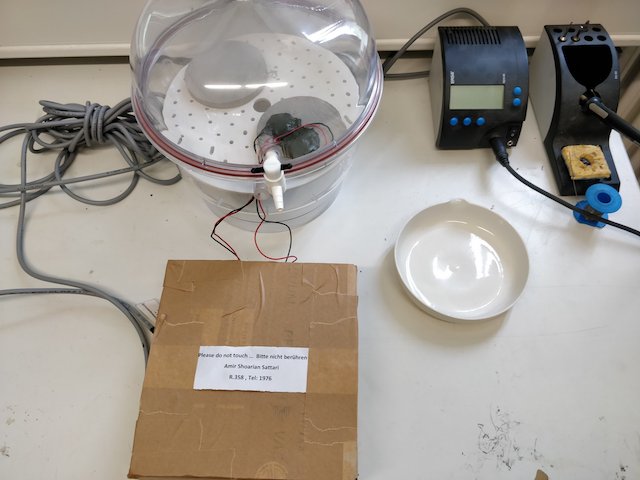
\includegraphics[width=1\textwidth]{figures/Amir_Shrinkage_Full_Setup.png}
\subcaption{}
\label{fig:Amir_Shrinkage_Full_Setup}
\end{subfigure}
\hfill
\begin{subfigure}[c]{0.48\textwidth}
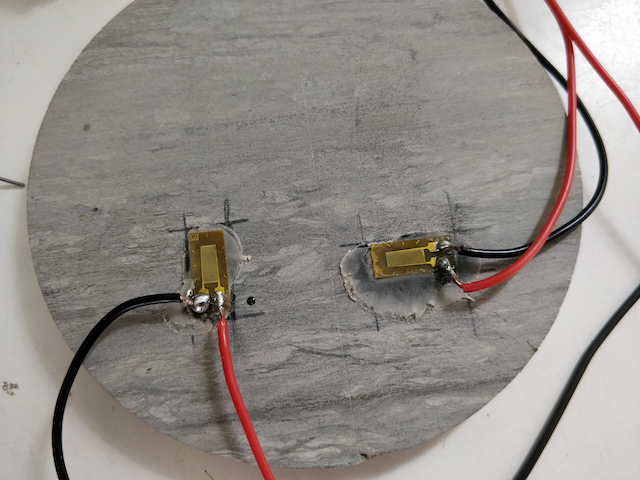
\includegraphics[width=1\textwidth]{figures/Amir_Shrinkage_Sensors.png}
\subcaption{}
\label{fig:Amir_Shrinkage_Sensors}
\end{subfigure}
\caption{The (a) desiccator setup, and (b) arraignment of the strain gauge strips on Opalinus claystone surface}
\end{figure}

The considered salt solution and its induced suction and relative humidity values in the constant room temperature of 20 $^{\circ}C$ are listed in Table \ref{table:Amir_Shrinkage_SaltSolutions}.

\begin{table}[h!]
\centering
\begin{center}
\begin{tabular}{ |>{\centering\arraybackslash}X m{7em}|>{\centering\arraybackslash}X m{10 em}|>{\centering\arraybackslash}X m{7em}|} 
\hline
Salt Solution & Relative Humidity (\%) & Suction ($MPa$) \\
\hline
$K_2SO_4$ & 97.6 & 3.2 \\
\hline
$KNO_3$ & 94.6 & 7.5 \\
\hline
$KCl$ & 85.1 & 21.8 \\
\hline
$NaCl$ & 75.5 & 38\\
\hline
$Mg(NO_3)_2$ & 54 & 84 \\
\hline
$MgCl_2$ & 33.1 & 149.5 \\
\hline
$LiCl$ & 12 & 286.7\\
\hline
$LiBr$ & 6.6 & 367.5\\
\hline
\end{tabular}
\end{center}
\caption{The saturated salt solutions relative humidity and suction values at 20 $^{\circ}C$}
\label{table:Amir_Shrinkage_SaltSolutions}
\end{table}

The samples dimension is 100x10 $mm$ $(DxL)$. The equilibrium inside the desiccator is reached when the change of the samples water content is equal to zero. Fig. \ref{fig:Amir_ME6_Strain} depicts the change of suction and axial linear strains in parallel and perpendicular directions. Similarly, Fig.\ref{fig:Amir_ME6_Water} shows the change of water content with applied suction using salt solutions. In drying path, the results indicate a higher strains for a strain perpendicular to the embedded layers. When the suction is higher than 150 $MPa$, the strains in perpendicular direction are almost 4.5 larger than parallel ones. Interestingly, in the wetting path, the differences between the strain gauges are much less. According to the water content data, the air-entry pressure for a sandy Opalinus claystone is around 25 $MPa$.

\begin{figure}[!ht]
\begin{subfigure}[b]{1\textwidth}
\centering
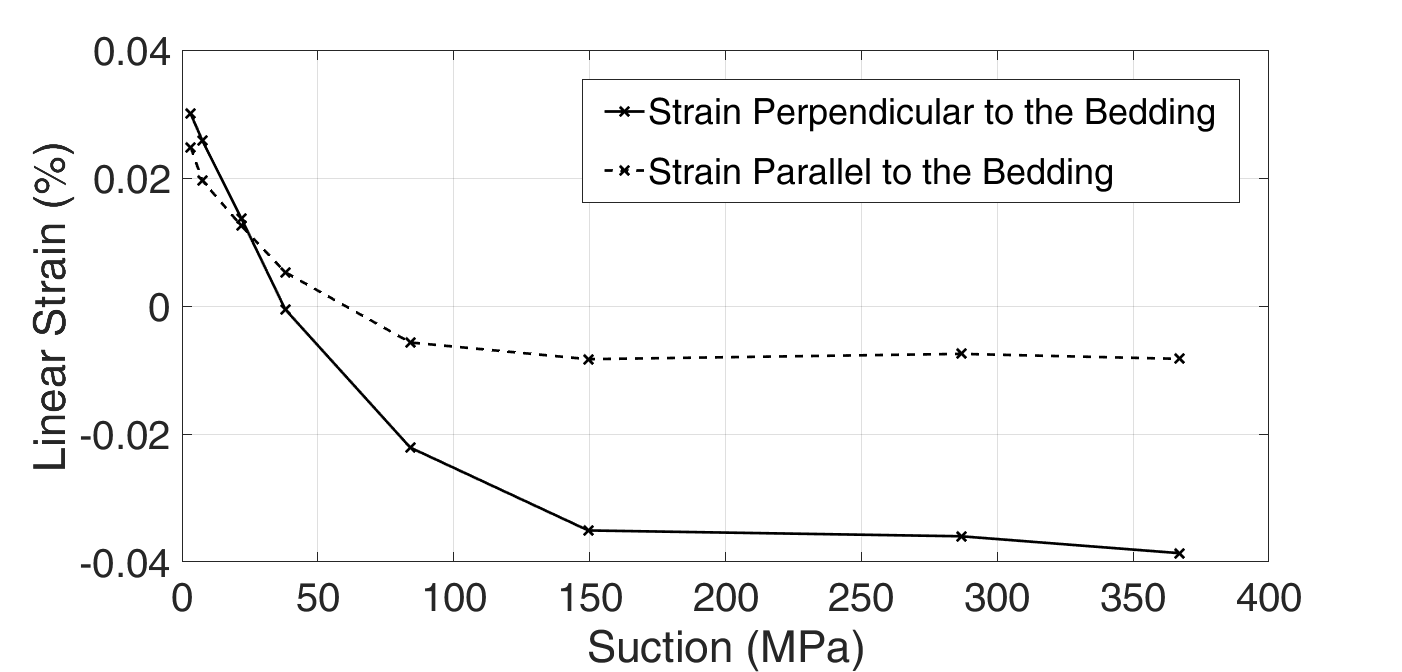
\includegraphics[width=11cm,height=6cm]{figures/Amir_ME6_Strain.png}
\subcaption{}
\label{fig:Amir_ME6_Strain}
\end{subfigure}
\\
\begin{subfigure}[b]{1\textwidth}
\centering
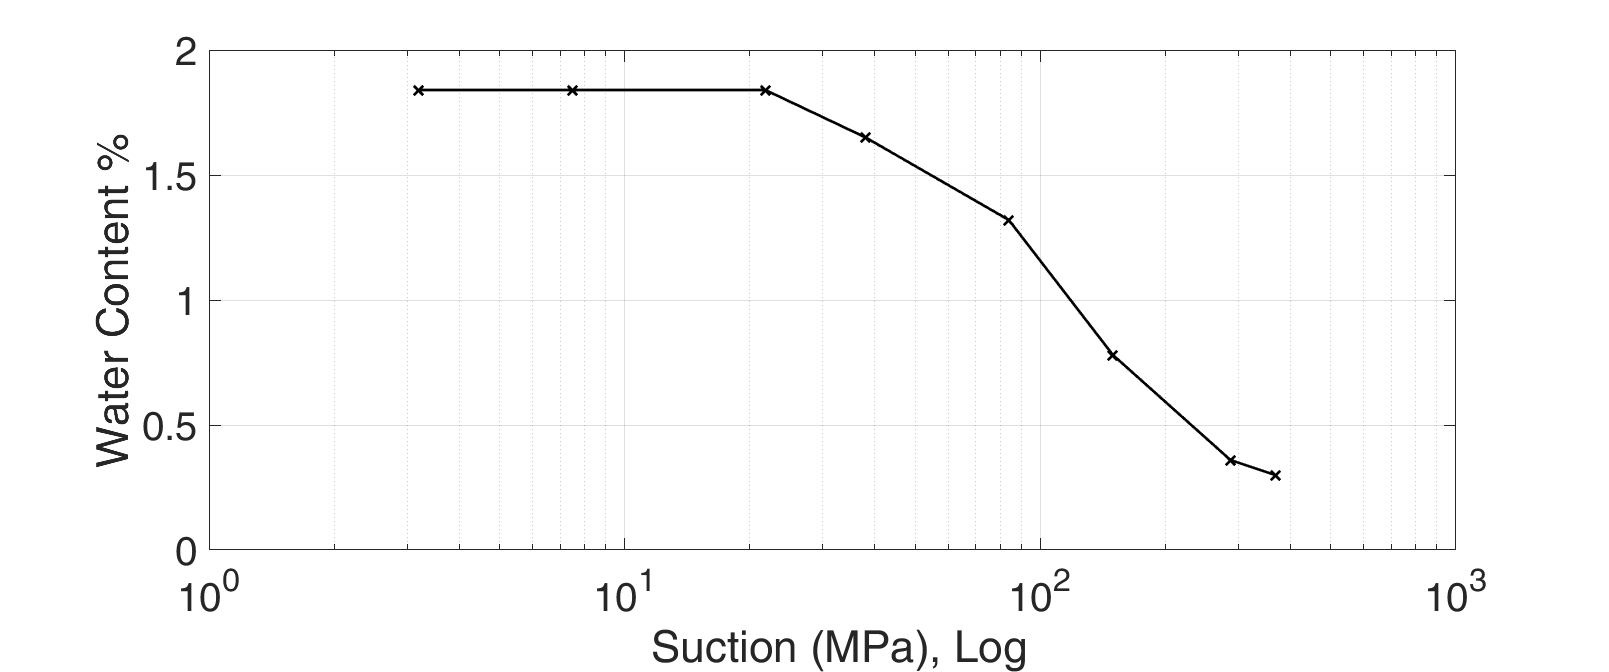
\includegraphics[width=11cm,height=6cm]{figures/Amir_ME6_Water.png}
\subcaption{}
\label{fig:Amir_ME6_Water}
\end{subfigure}
\caption{The drying and wetting paths for Opalinus claystone (a) the suction vs. linear strains, and (b) the suction vs. the water content}
\end{figure}


%------------------------------------------------------------------------------
\subsection{Model approaches}

The simulation results from both of the model methods, lattice element method (LEM) and variational phase field model (VPF), are described and the accuracy of numerical results for modeling the shrinkage process with change of linear or volumetric strains as well as the change of anisotropic hydraulic conductivity are investigated. 

\subsubsection*{Lattice element model}

With the application of the integrated interface element \cite{Sattarietal2019b} the drying and wetting processes in the Opalinus claystone are simulated. The linear strain of the elements are calculated based on the experimental data. The initial hydraulic conductivity ($k_h$) values are approximated according to the technical Report, Mont Terri 2008-04 as,

\begin{align}
\label{eq:LEM_ME6_1}
\begin{split}
k_{h,\parallel}=2\times{10}{^{-13}}
\quad , \quad
k_{h,\bot}=0.6\times{10}{^{-13}}
\end{split}
\end{align}

While considering the cubic law for flow transfer through the porous medium, the hydraulic aperture or length of the interface element is calculated as,

\begin{align}
\label{eq:LEM_ME6_2}
\begin{split}
a_h=\sqrt{\frac{12k_h\nu_f}{g}}
\quad , \quad
a_{h,\parallel}=4.95\times{10}{^{-10}}
\quad , \quad
a_{h,\bot}=2.71\times{10}{^{-10}}
\end{split}
\end{align}

where $\nu_f=1.004\times{10}{^{-6} [m^2.s^-1]}$ and $g=9.8$. The domain is generated using the vectorizable lattice element with defined layers as described in previous sections (Fig. \ref{fig:Amir_ME6_Lattice_Setup}). The interface length is defined based on Eq. \ref{eq:LEM_ME6_2}. The interface strength between two layers is assumed to be 5 times weaker than the bond between a same layer. Therefore, fracking along the layers in X and Z directions is expected, Which results in higher hydraulic conductivity values as the wetting and drying process continues (Fig. \ref{fig:Amir_ME6_Lattice_Frack}). Fig. \ref{fig:Amir_ME6_Lattice_Drying}) depicts the change of hydraulic conductivity along three axis of X, Y and Z. As expected, the change of the hydraulic conductivity during the drying process is the lowest along the Y axis, where the drying process is perpendicular to the embedded layering orientation. 

\begin{figure}[!ht]
\begin{subfigure}[c]{0.5\textwidth}
\centering
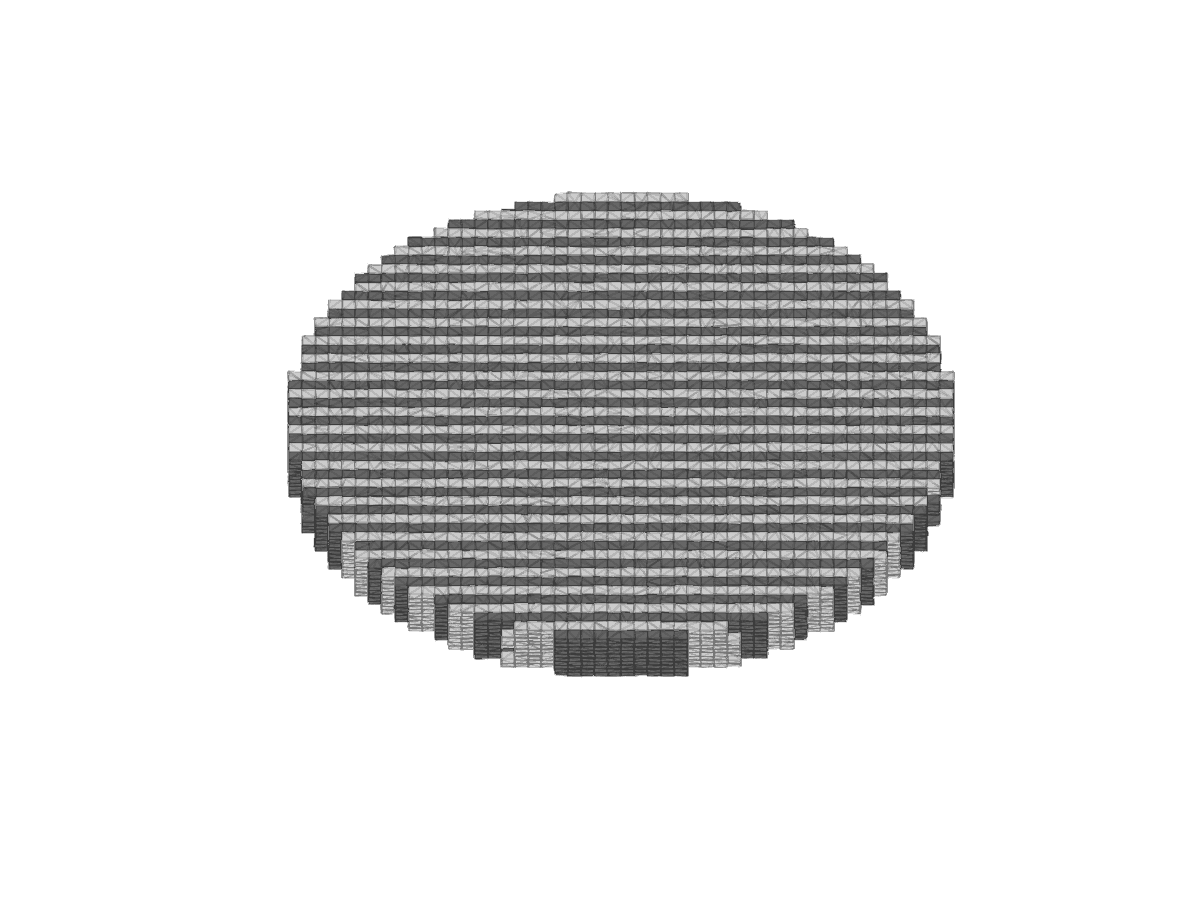
\includegraphics[width=5cm,height=5cm]{figures/Amir_ME6_Lattice_Setup.png}
\subcaption{}
\label{fig:Amir_ME6_Lattice_Setup}
\end{subfigure}
\begin{subfigure}[c]{0.5\textwidth}
\centering
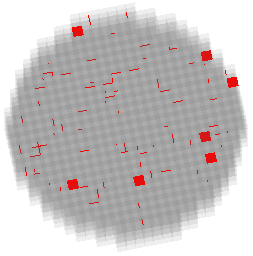
\includegraphics[width=5cm,height=5cm]{figures/Amir_ME6_Lattice_Frack.png}
\subcaption{}
\label{fig:Amir_ME6_Lattice_Frack}
\end{subfigure}
\caption{The (a) generated domain for simulation of the drying and wetting processes, and (b) fracking paths shown with red surfaces}
\end{figure}


\begin{figure}[!ht]
\centering
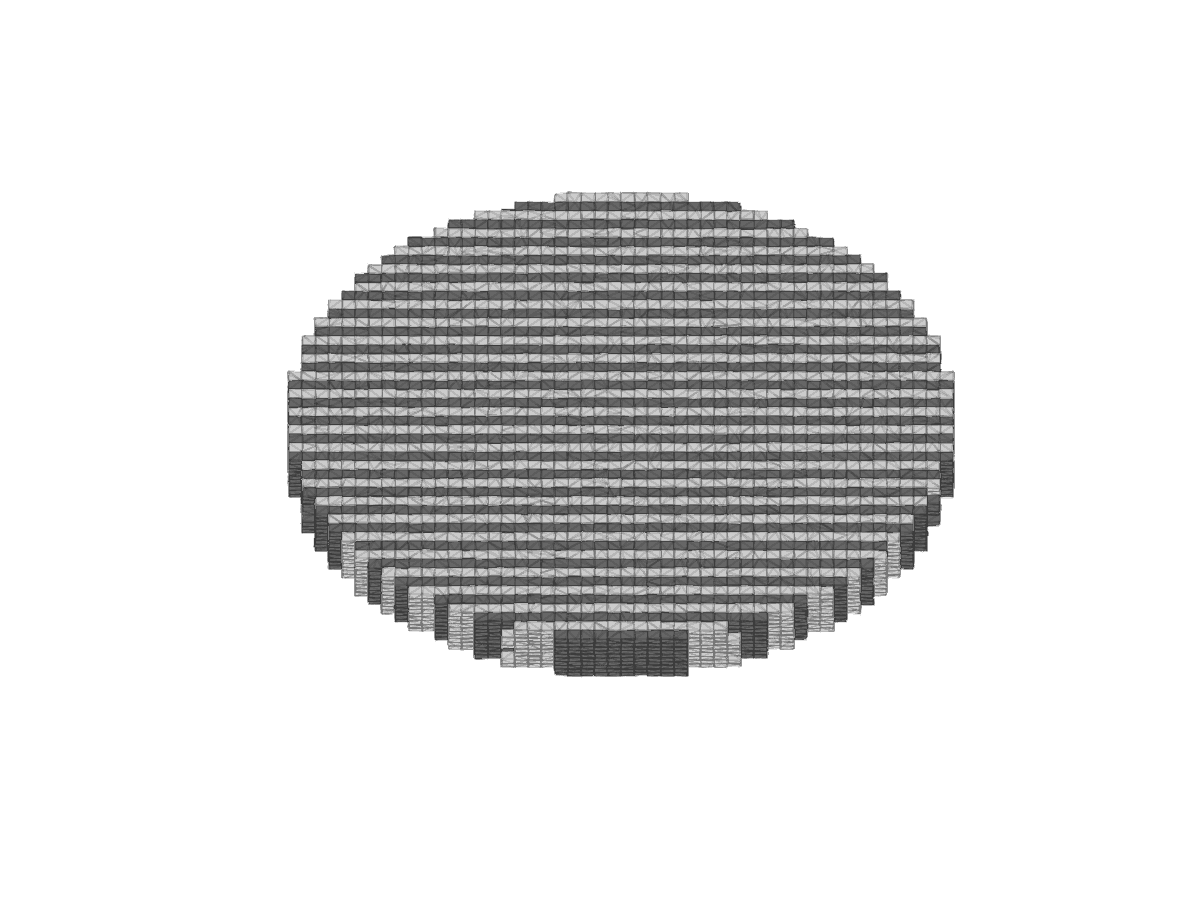
\includegraphics[width=8cm,height=5cm]{figures/Amir_ME6_Lattice_Setup.png}
\caption{The change of hydraulic conductivity along three axis for Opalinus claystone under drying process}
\label{fig:Amir_ME6_Lattice_Drying}
\end{figure} 


%-----------------------------


\subsubsection*{Finite-Element-Method: Variational-Phase-Field (VPF)}
While couplnng of unsaturated flow (Richards flow) and variational phase-field based formulation of fracture mechanics is underway in OGS, the contribution from VPF is being planned. 
Once the model becomes available, strain changes driven by shrinkage or swelling of the sample which is subject to the pore--pressure and the partial saturation changes is modeled utilizing the current Richard--Mechanics implementation in OGS. Then desiccation cracking will be simulated through the variational phase-field using the strain energy contributed from the shrinkage and swelling.
A tentative FEM mesh prepared is shown in~\ref{fig:ME5_VPF_setup}.
The alternating hydraulic conductivities and the material strength will need to be assigned accordingly to the LEM simulation.

\begin{figure}[!ht]
\centering
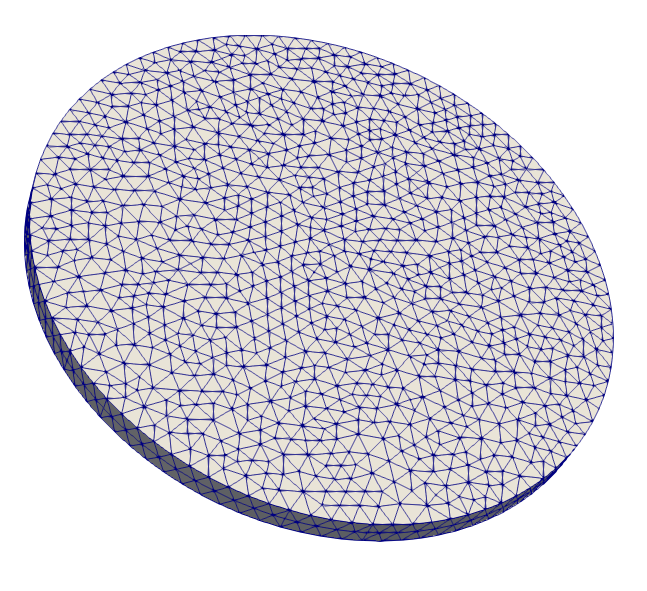
\includegraphics[width=0.75\textwidth]{figures/ME5_VPF_mesh.png}
\caption{The generated FEM mesh for shrinkage process}
\label{fig:ME5_VPF_setup}
\end{figure} 
%------------------------------------------------------------------------------
\subsection{Results and discussion}

The experimental data assessed during the drying and wetting processes confirms the high anisotropy of Opalinus claystone. Using the saturated salt solutions to apply the osmotic suction, the change of water content as well as the micro deformations along two axis (parallel and perpendicular) are captured and recorded. Higher anisotropy factors during the drying path than in wetting path is observed (Fig. \ref{fig:Amir_ME6_Strain}). The initial water content of the sample was lower than expected in the literature, mainly due to the sample preparation process, where the sample was subjected to the different relative humidity. Fig. \ref{fig:Amir_ME6_Water} shows the air-entry pressure to be around 25 $MPa$. similarly, the residual pressure corresponding to the residual water content is found to be 180 $MPa$ (for more information regarding the soil-water retention curves see \hl{cite Sattarietal2020}. The numerical lattice model to simulate the drying and wetting paths is implemented and with defining the anisotropy, the change of the hydraulic conductivity along different axis is determined. The results show a similar behavior as seen from experimental data. However, more quantitative comparison of the data between experimental and numerical results is required. 